\chapter{Oasis Lib}
\label{ch:Lib}
In this chapter we describe the Oasis Lib.
The Oasis Lib is the library, which works as a connection between the Oasis Local Db, see Section \vref{ch:Db}, and the GIRAF applications.
The Oasis Lib provides an API, which the GIRAF applications can use.
The structure of the Oasis Lib is described in Section \vref{sec:Structure}.
Finally the implementation of the Oasis Lib is described in Section \vref{sec:LibImp}.

\section{Structure}
\label{sec:Structure}
The structure of the Oasis Lib, have been inspired of the MVC pattern, where the system is divided into three parts; Model, View, and Controller. 

In Oasis Lib the Model part is a package containing model classes. Each model class represents a table in the Oasis Local Db.
The model classes are used to encapsulate the data, which is to be stored and retrieved from the Oasis Local Db.
The reason that we use model classes is to ease it for the users of the library and to make a uniform way of storing and retrieving data.
The model classes can be seen in Figure \vref{fig:models}.
\begin{figure}[H]
	\centering
		\includegraphics[width=0.5\textwidth]{images/models.png}
	\caption{The models in the Oasis Lib}
	\label{fig:models}
\end{figure}

The Controller part is the package containing all the methods, which the developers can use to interact with Oasis Local Db.
The controller methods have been divided into several classes.
The division can be seen in Figure \vref{fig:controllers}.
\begin{figure}[H]
	\centering
		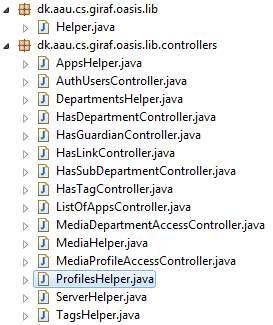
\includegraphics[width=0.5\textwidth]{images/controllers.png}
	\caption{The controllers in the Oasis Lib}
	\label{fig:controllers}
\end{figure}

The controllers are divided by the models they manipulate, this means that for each table in the Oasis Local Db there is a controller.

In the Oasis Lib there is no direct reference to the Views from the MVC pattern.
This is because the individual applications in the GIRAF system is seen as a view.

\section{Implementation}
\label{sec:LibImp}
The Oasis Lib has been designed with the intention of having as few method calls as possible to gain access to the Oasis Local Db.
The code for all the implemented methods will not be show in this section.
Two examples from the Oasis Lib will be presented, these methods are \texttt{autenticateProfile} and \texttt{getProfileById}.


The method \texttt{autenticateProfile} is used to authenticate a profile in order to decide what informations the user should be allowed access to.

First the method verifies that the input is not \texttt{null} and that the certificate conformes to the rules for the certificates, if the certificate is rejected, \texttt{null} is returned to indicate this.

After the certificate has been verified the profile id will be retrived from the Oasis Local Db, iff a profile exists with that certificate.
In case a profile exist with the certificate the id will be returned and the profile model will be retrieved from the Oasis Local Db.
If no profile with the certificate exists, \texttt{-1} will be returned and no profile model will be retrieved.

The code for \texttt{autenticateProfile} can be seen in Listing \vref{lst:authenticateProfile_implementation}.

\begin{Java}{The \texttt{authenticateProfile} method.}{lst:authenticateProfile_implementation}
public Profile authenticateProfile(String certificate) {
	if (certificate == null || !certificate.matches("[a-z]{200}")) {
		return null;
	}

	Profile profile = null;
	long id = au.getIdByCertificate(certificate);

	if (id != -1) {
		profile = getProfileById(id);
	}

	return profile;
}
\end{Java}

The method \texttt{getProfileById} is used the retrieve a profile model from the database.
The model is retrived using the profile id as a parameter to get the model by.

First it must be ensured that the id is above zero, as the database can not handle zero or negative values.
After this check the database is queried to retrive the profile model.
A conversion is needed as the database returns a Cursor object and this object must be converted into a profile model. \cite{Cursor}
This conversion is done in the auxiliary method \texttt{cursorToProfile}, which maps values in the Cursor to values in the profile model.
If the Cursor from the database is null or empty, no profile was found in the database.

The code for \texttt{getProfileById} method can be seen in Listing \vref{lst:getProfileById_implementation}.

\begin{Java}{The \texttt{getProfileById} method.}{lst:getProfileById_implementation}
public Profile getProfileById(long id) {
	Profile profile = null;
	
	if (id <= 0) {
		return null;
	}
	
	Uri uri = ContentUris.withAppendedId(ProfilesMetaData.CONTENT_URI, id);
	Cursor c = _context.getContentResolver().query(uri, columns, null, null, null);

	if (c != null) {
		if (c.moveToFirst()) {
			profile = cursorToProfile(c);
		}
		c.close();
	}

	return profile;
}
\end{Java}

For further information on how the Oasis Lib methods work, see the JavaDoc or the source code, which are placed on the attached CD-ROM. 